% Experiments

This section presents the experiments and results aimed at evaluating our proposed graph generative model. First we run a grid-search on the hyperparameter space to find the optimal configuration of the RGVAE. We use the ELBO and MRR as evaluation metric. The best configurations are used to perform link prediction. Here we compare the model performance with vs. without convolutions. We use the VDistMult as control model for link prediction. Finally we run two proof-of-concept experiments. The first generating triples and filter on a entity class constraining relation, thus we get an insight of how much percent of the generated triples are valid. Secondly we analyze the results of a RGVAE trained on subgraphs with $n=10$. For the experiments we use two multi-relational KG datasets.

% We covered link and node prediction and compared those to SOTA scores. Further we ran experiments on investigating the coherence of the reproduced graph structure. Lastly we measured the adherence of our model to the KG's underlying syntax.


\subsection{Data}
For this sake of comparison with state of the art results, we chose the two most popular dataset used in this field of KG link prediction, FB15k237 and WN18rr.

% Training models on each dataset for 333 epochs, without early stopping.

\textbf{Fb15k-237}

\printinunitsof{in}\prntlen{\textwidth}


This dataset is a subset of the FreeBase KG (cite).[Explain Free Base] The original Fb15k had redundant triples, creating ambiguity during training. In the updated version, Fb15k-237, these triples were removed what led to a more robust dataset, which is commonly used as benchmark for several NLP tasks.

% or/and
A subset from one of the first and largest KGs, called FreeBase. In the first version of this dataset, it was possible to infer most of the test triples by inverting triples in the trainset, Thus the latest $237$ version filtered these triples out.
The dataset contains $14,951$ entities and $1,345$ different relations.

\textbf{WN18rr}

Based on the wordnet KG.

% Table comparing numbers

\subsection{Hyperparameter Tuning}

In this section we run a grid search for the three hyperparameters $\beta$, $d_z$ and $d_h$ for a set of contrastive values. To reduce the computational expenses we train each model for $60$ epochs and  evaluate link prediction on a subset of $50$ triples.

Empirically we set the learning rate to $3e-5$ and the batchsize to the maximum fir on the GPU memory. For $d_h$ we did not see any significant changes for higher values, thus we choose a lower number to reduce the total model parameters. The remaining hyperparameter did influence and the optimal setting vary for each dataset, table \Ref shows the results of our hyperparameter tuning.

% lr empirically and batchszize fixed.

% beta
We compare the values of $\beta \in [0,1,10,100]$

\begin{figure}[H]
    \centering
    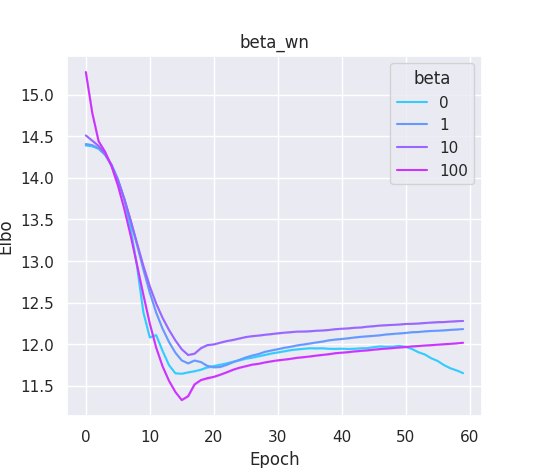
\includegraphics[width=0.5\textwidth]{graphs/plots/beta_wn.png}
    \label{fig5:betawn}
\end{figure}

% d_z

% d_h did not influcence

RGVAE:
hidden dimensions
latent dimensions
beta


RGCVAE


\subsection{Link Prediction}
% The task of link prediction, tests, if the model can recognize the relation between two entities. In order to do so, we hide the second entity of a triple and let our model to predict it.

% We used link prediction as evaluation protocol and for comparison state of the art models. For each triple in the dataset, we remove the tail and combine it with all possible entities in our dataset. EVen though this is called 'triple-corruption', also correct triples can be generated, which could appear in the trainset. These have bo the filtered out before evaluation. Link prediction on unfiltered test data is termed 'raw'. Our model then computes the ELBO loss for all corrupted triples, which are sorted and stored in ascending order. The same procedure is repeated the triple's head in place of the tail.


% The metrics used to evaluate the predictions, is the mean reciprocal rank (MRR) and hits at 1,3 and 10.
% The MRR ??? explain what the MRR is.

% Hits at 1 indicates what percentage of the triples in the test set have been ranked the highest compared to their corruptions. Similar, hits at 3 and 10, give a percentage of triples ranked in the top 3 and top 10.
% These metrics allow a fair comparison on a dataset between models, regardless of the ranking method of each model.



% Evaluation protocol For evaluation, we use the same ranking procedure as in [3]. For each test
% triplet, the head is removed and replaced by each of the entities of the dictionary in turn. Dissimilarities (or energies) of those corrupted triplets are first computed by the models and then sorted by
% ascending order; the rank of the correct entity is finally stored. This whole procedure is repeated
% while removing the tail instead of the head. We report the mean of those predicted ranks and the
% hits@10, i.e. the proportion of correct entities ranked in the top 10.
% These metrics are indicative but can be flawed when some corrupted triplets end up being valid
% ones, from the training set for instance. In this case, those may be ranked above the test triplet, but
% this should not be counted as an error because both triplets are true. To avoid such a misleading
% behavior, we propose to remove from the list of corrupted triplets all the triplets that appear either in
% the training, validation or test set (except the test triplet of interest). This ensures that all corrupted
% triplets do not belong to the data set. In the following, we report mean ranks and hits@10 according
% to both settings: the original (possibly flawed) one is termed raw, while w


% We use negative elbo as scoring function. Since elbo is aimed to be reduced and LP scores are higher better.

We try with and without permutation

We try the model as encoder only

We use 1/3 of the test set only, randomly drawn. Run 3 times?
Final models only 60 epochs



Different models
Report:
loss converges
MRR stays almost zero

With vs. w/o graph matching


\subsubsection{DistMult lp}
To find out why our model fails to perform lp we run the original DistMult with optimal parameters from \cite{ruffinelli_you_2019} and a variational DistMult version, which samples from a latent distribution, just like the VAE. Give implementation link.

Answer question:Link prediction with control model:
Distmult vs Var Distmult

We see that the variational part messes everything up.

Graphs:
MRR + Hits@all + Loss

\subsection{Impact of permutation}
% Check if adj matrix adheres to edge attribute matrix.

Graph of permutation during training
loss with vs without 

\subsection{Interpolate Latent Space}
We take two random triples and interpolate the latent space of these two triples. The interpolations result in: HERE AN EXAMPLE.

Further we go ahead and test what happens if we modify one latent dimension of a triple. HERE AN EXAPMPLE.

Can the model assign logical features to latent dimensions?


\subsection{Syntax coherence}

Check model trained with vs without perm invariance.

Check if generated triples follow basic logic.
\begin{itemize}
    \item Generate triples by random signals
    \item Filter these triples on a certain relation
    \item Check if the entities are part of the linked class
\end{itemize}

Since there is no preset for how to check the semantics of a KG, we will use simple basic logical criteria.
The generated triples are filtered for the relation 'is capital of', thus the subject entity should be a city and he object entity member of the class 'country',
Hope this gives good results.


\subsection{Subgraph Generation}
Until now our model trained on only one triple per sparse graph. What will happen if we train it on more than one triples?
